% Purpose: Generalized scientific article template for
% evidence-bounded technical
% communication, including methods, reproducibility, results, and limitations.
% Status: Draft; author, venue, citations, data, and human review pending.
% Source-of-truth: [Repository-relative source, schema, test, and data paths]
\documentclass[10pt,a4paper]{article}

% -----------------------------------------------------------------------------
% Document configuration
% -----------------------------------------------------------------------------
\usepackage[margin=2.0cm]{geometry}
\usepackage[T1]{fontenc}
\usepackage[utf8]{inputenc}
\usepackage{lmodern}
\usepackage{microtype}
\usepackage{amsmath,amssymb}
\usepackage{booktabs}
\usepackage{tabularx}
\usepackage{threeparttable}
\usepackage{siunitx}
\usepackage{array}
\usepackage{enumitem}
\usepackage{xcolor}
\usepackage{tikz}
\usetikzlibrary{arrows.meta,positioning,calc,fit,backgrounds,shapes.geometric,shapes.misc}
\usepackage{pgfplots}
\pgfplotsset{compat=1.18}
\usepackage{hyperref}
\usepackage{cleveref}

\hypersetup{
  colorlinks=true,
  linkcolor=black!70,
  citecolor=blue!60!black,
  urlcolor=blue!70!black,
  pdftitle={Scientific Article Template},
  pdfauthor={[Author name]}
}
\sisetup{
  detect-all,
  round-mode=places,
  round-precision=2,
  group-separator={,},
  input-symbols = (),
  table-number-alignment = center
}
\setlist{nosep,leftmargin=*}
\setlength{\parindent}{0pt}
\setlength{\parskip}{4pt}
\newcolumntype{Y}{>{\raggedright\arraybackslash}X}

% Semantic operators and document-specific notation.
\DeclareMathOperator{\argmin}{arg\,min}
\DeclareMathOperator{\diag}{diag}
\newcommand{\projectname}{[Project name]}
\newcommand{\statusplanned}{[Planned]}
\newcommand{\statusimplemented}{Implemented}
\newcommand{\statusobserved}{Observed}
\newcommand{\statusderived}{Derived}
\newcommand{\statussynthetic}{Observed (Synthetic)}
\newcommand{\unitlabel}[1]{\mathrm{#1}}

% Evidence-status styles: solid demonstrated code, double persistence, and
% dashed roadmap components remain visually distinct in diagrams.
\tikzset{
  >=Stealth,
  template node/.style={
    rectangle, rounded corners=2pt, draw=black!80, line width=0.7pt,
    align=center, inner sep=5pt, minimum height=9mm, text width=31mm
  },
  implemented node/.style={template node, fill=blue!8, draw=blue!70!black},
  persistence node/.style={
    template node, fill=gray!12, draw=black!80, double, double distance=1pt
  },
  human node/.style={
    template node, chamfered rectangle, fill=orange!12, draw=orange!80!black
  },
  planned node/.style={
    template node, fill=gray!5, draw=black!50,
    dash pattern=on 3.5pt off 2.5pt, font=\small\itshape
  },
  template arrow/.style={->, thick, draw=black!75},
  planned arrow/.style={->, thick, dashed, draw=black!50}
}

% -----------------------------------------------------------------------------
% Metadata: replace bracketed fields and verify every claim against its source.
% -----------------------------------------------------------------------------
\title{\projectname\\
\large[Specific scientific or engineering contribution]}
\author{[Author One]\\
  \small[Institution, city, country]\\
\small\href{mailto:[author@example.org]}{[author@example.org]}}
\date{[Month Day, Year]}

\begin{document}
\maketitle

% Abstract contract: problem, method, demonstrated result, and scope boundary.
\begin{abstract}
  [State the problem and why it matters.] [State the data, method, or system
  studied.] [Report only verified results, with sample bounds and uncertainty
  where available.] [State the principal limitation and do not imply that
  planned or synthetic components are empirical findings.]
\end{abstract}

\textbf{Keywords:} [keyword one]; [keyword two]; [keyword three];
[reproducibility term]

% -----------------------------------------------------------------------------
\section{Introduction and Motivation}
% -----------------------------------------------------------------------------
[Define the domain problem, the intended audience, and the gap addressed by
  this document. Distinguish the motivating hypothesis from results
  demonstrated
by the present implementation or experiment.]

The document makes the following bounded contributions:
\begin{enumerate}
  \item [Contribution anchored in a source file, protocol, or approved record.]
  \item [Deterministic method or system capability, with its
    verification test.]
  \item [Empirical observation or derived statistic, with dataset version and
    sample bounds.]
\end{enumerate}

\textbf{Scope boundary.} [List capabilities that are planned, hypothetical,
  or outside the evaluated scope. Do not describe them with the same certainty
or visual treatment as demonstrated components.]

% -----------------------------------------------------------------------------
\section{Scientific and Theoretical Foundations}
% -----------------------------------------------------------------------------
[Introduce the relevant theory and literature baselines. Define every symbol
  when it first appears, including its domain and units. Explain
  which equations
  are literature definitions, which are implemented algorithms, and which are
hypotheses or proposed extensions.]

Let $i \in \mathcal{I}$ index an entity in the finite entity set
$\mathcal{I}$, let $t \in \mathcal{T}$ index an observation period in the
finite ordered set $\mathcal{T}$, and let $x_{i,t} \in \mathbb{R}$ denote the
observed value for entity $i$ at period $t$ in the stated measurement unit.
For a non-empty matched set $\mathcal{M}_t \subseteq \mathcal{I}$, a generic
arithmetic relative statistic is
\begin{equation}
  R_t = \frac{1}{|\mathcal{M}_t|}
  \sum_{i \in \mathcal{M}_t}
  \frac{x_{i,t}}{x_{i,t_0}},
  \qquad
  \mathcal{M}_t \subseteq \mathcal{I},\quad
  1 \leq |\mathcal{M}_t| \leq |\mathcal{I}|,
  \quad x_{i,t_0} > 0.
\end{equation}
Here $t_0 \in \mathcal{T}$ is the explicitly declared base period, and
$|\mathcal{M}_t|$ is the number of valid matched entities. This equation is a
template only: replace it with the exact implemented computation and cite the
source module or test that verifies it.

If a weighted estimator is used, define weights $w_i \in \mathbb{R}_{\geq 0}$
for every $i \in \mathcal{I}$ and state the normalization constraint
$\sum_{i\in\mathcal{I}} w_i = 1$. For uncertainty, define the estimator,
resampling unit, confidence level $\alpha \in (0,1)$, and interval procedure;
do not add uncertainty bounds merely because they appear in a literature
formula.

% -----------------------------------------------------------------------------
\section{Data, Materials, and Provenance}
% -----------------------------------------------------------------------------
[Describe the data-generating process, inclusion and exclusion rules, version,
  access restrictions, units, missingness, and ethical or privacy
  controls. Mark
  each input as observed empirical data, observed synthetic data, or a planned
  input. A repository-relative path, checksum, release identifier, or approved
record should anchor each material.]

\begin{table}[htbp]
  \centering
  \small
  \caption{Data dictionary and evidence classification for the analysis inputs.
    Replace each placeholder with the exact field name, domain constraint, and
  source anchor; rows marked synthetic are not empirical observations.}
  \label{tab:data-dictionary}
  \begin{threeparttable}
    \begin{tabularx}{\linewidth}{l l X l X}
      \toprule
      \textbf{Field} & \textbf{Type} & \textbf{Domain / constraint} &
      \textbf{Evidence} & \textbf{Operational meaning and source anchor} \\
      \midrule
      \texttt{[field\_raw]} & String & [Non-empty or permitted missing value] &
      \statusobserved & [Primary input; path or schema] \\
      \texttt{[field\_normalized]} & String & [Controlled vocabulary
      or mapping] &
      Analyst-normalized & [Mapping rule; reviewer or version] \\
      \texttt{[measurement]} & Float & [Unit and finite domain, e.g. $>0$] &
      \statusobserved & [Instrument or collection protocol] \\
      \texttt{[derived\_metric]} & Float & [Formula and valid range] &
      \statusderived & [Algorithm and test anchor] \\
      \bottomrule
    \end{tabularx}
    \begin{tablenotes}[flushleft]
      \footnotesize
    \item Evidence labels distinguish raw observations, analyst
      normalizations, and deterministic derived metrics. State the dataset
      version, physical units, currency, and missing-value convention here.
    \end{tablenotes}
  \end{threeparttable}
\end{table}

% -----------------------------------------------------------------------------
\section{System Architecture and Methodology}
% -----------------------------------------------------------------------------
[Describe the executable pipeline in dependency order. Name the module,
  configuration, schema, or protocol controlling each step. Explain where human
review enters and how provenance is preserved.]

\begin{figure}[htbp]
  \centering
  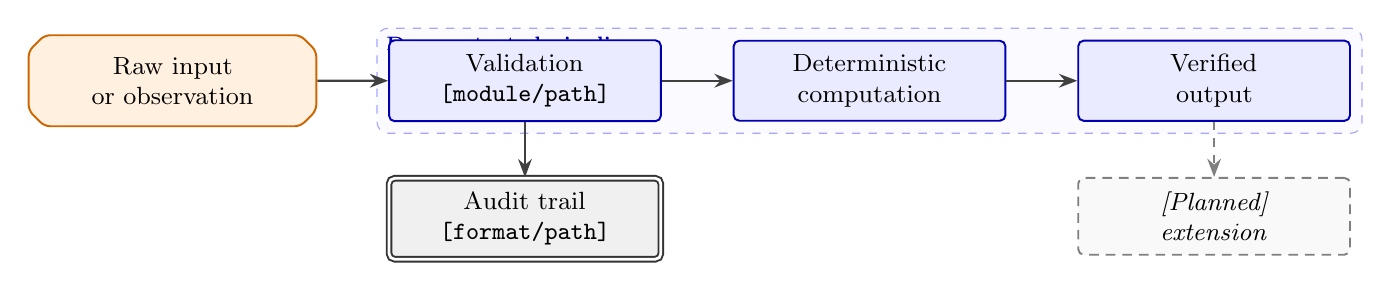
\begin{tikzpicture}[node distance=7mm and 9mm, every
    node/.style={font=\small}]
    \node[human node] (input) {Raw input\\or observation};
    \node[implemented node, right=of input] (validate)
    {Validation\\\texttt{[module/path]}};
    \node[persistence node, below=of validate] (ledger) {Audit
    trail\\\texttt{[format/path]}};
    \node[implemented node, right=of validate] (compute)
    {Deterministic\\computation};
    \node[implemented node, right=of compute] (result) {Verified\\output};
    \node[planned node, below=of result] (future) {[Planned]\\extension};

    \draw[template arrow] (input) -- (validate);
    \draw[template arrow] (validate) -- (compute);
    \draw[template arrow] (validate) -- (ledger);
    \draw[template arrow] (compute) -- (result);
    \draw[planned arrow] (result) -- (future);

    \begin{pgfonlayer}{background}
      \node[draw=blue!35, fill=blue!2, dashed, rounded corners=4pt,
      fit=(validate) (compute) (result), inner sep=4pt] (pipeline) {};
      \node[anchor=north west, font=\scriptsize\bfseries\color{blue!65!black}]
      at (pipeline.north west) {Demonstrated pipeline};
    \end{pgfonlayer}
  \end{tikzpicture}
  \caption{Evidence-aware architecture for the [system or analysis name]. The
    reader should distinguish human inputs, executable modules,
    persistence, and
    the dashed planned extension. Solid nodes must be anchored in
    tested source;
    this template diagram contains no empirical result and requires
    project-path
  replacement.}
  \label{fig:architecture}
\end{figure}

\subsection{Algorithm and implementation binding}
[Give pseudocode or a short ordered description only when it clarifies the
  implementation. For each parameter, state its default, allowed domain, and
  source of truth. Explain failure behavior, invalid-input handling,
  and whether
the operation mutates source data.]

% -----------------------------------------------------------------------------
\section{Experimental Protocol and Reproducibility}
% -----------------------------------------------------------------------------
[State the research question, design, baselines, comparison unit, random seed,
  software versions, hardware, stopping rule, and evaluation
  metrics. Separate a
  planned protocol from a completed run. Do not call a fixture a
  benchmark unless
its provenance and comparison basis are stated.]

\begin{enumerate}
  \item \textbf{Preparation:} [Dataset version, preprocessing, and exclusions.]
  \item \textbf{Execution:} \texttt{[exact command or workflow entry point]}
    with [configuration and seed].
  \item \textbf{Evaluation:} [Metric definition, denominator, units, and
    uncertainty or repeat policy].
  \item \textbf{Preservation:} [Output path, log, checksum, or review record.]
\end{enumerate}

% -----------------------------------------------------------------------------
\section{Results}
% -----------------------------------------------------------------------------
[Report only completed runs. Give sample size $N \in \mathbb{Z}_{>0}$, dataset
  version, baseline, unit, precision rationale, and uncertainty
  where available.
A null, missing, or unsupported result should remain visible.]

\begin{table}[htbp]
  \centering
  \small
  \caption{Results template for a bounded comparison. Values are placeholders
    and must be replaced by outputs reproduced from the stated protocol; the
  synthetic row is illustrative and is not an empirical claim.}
  \label{tab:results}
  \begin{threeparttable}
    \begin{tabularx}{\linewidth}{l S S X l}
      \toprule
      \textbf{Condition} & {\textbf{Metric}} & {\textbf{Uncertainty}} &
      \textbf{Interpretation} & \textbf{Evidence} \\
      \midrule
      [Baseline] & 0.00 & 0.00 & [Reference condition and units] &
      [Observed / derived] \\
      [Method A] & 0.00 & 0.00 & [Difference from baseline; no causal claim] &
      [Derived] \\
      [Synthetic fixture] & 0.00 & 0.00 & [Executable check only] &
      [\statussynthetic] \\
      \bottomrule
    \end{tabularx}
    \begin{tablenotes}[flushleft]
      \footnotesize
    \item Report $N$, metric definition, unit, baseline, dataset or fixture
      version, and the test or run record. Use ``not available'' when a value
      was not measured; never replace it with zero.
    \end{tablenotes}
  \end{threeparttable}
\end{table}

\begin{figure}[htbp]
  \centering
  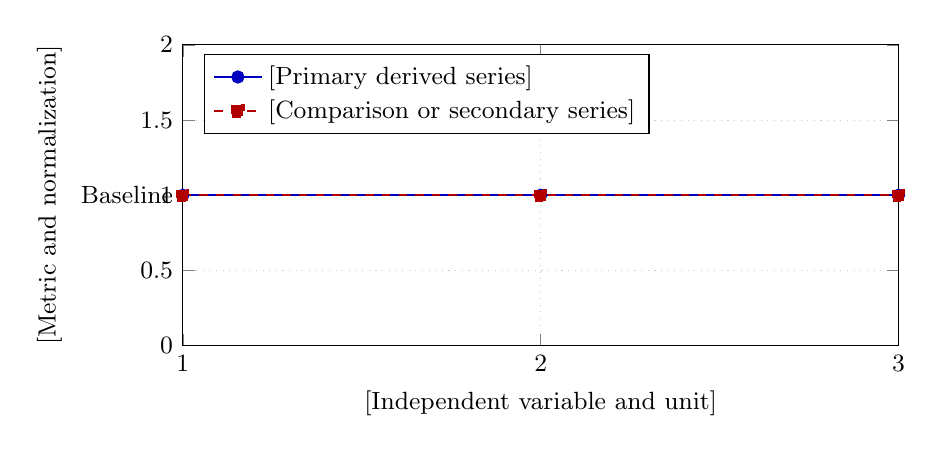
\begin{tikzpicture}
    \begin{axis}[
        width=0.88\linewidth,
        height=5.4cm,
        xlabel={[Independent variable and unit]},
        ylabel={[Metric and normalization]},
        xmin=1, xmax=3,
        ymin=0, ymax=2,
        xtick={1,2,3},
        extra y ticks={1},
        extra y tick labels={Baseline},
        extra y tick style={grid=major, grid style={dashed, black!55}},
        grid=both,
        grid style={dotted, gray!40},
        legend pos=north west,
        legend cell align={left},
        font=\small
      ]
      % Replace placeholder coordinates with verified output values.
      \addplot[thick, blue!75!black, mark=*] coordinates {
        (1, 1.00) (2, 1.00) (3, 1.00)
      };
      \addlegendentry{[Primary derived series]}
      \addplot[thick, red!70!black, dashed, mark=square*] coordinates {
        (1, 1.00) (2, 1.00) (3, 1.00)
      };
      \addlegendentry{[Comparison or secondary series]}
    \end{axis}
  \end{tikzpicture}
  \caption{Quantitative trajectory for [metric and dataset]. The
    dashed baseline
    makes the reference value explicit and the two series separate primary from
    comparative output. Coordinates are illustrative placeholders, not a
    measured result; replace them with verified values, sample
    bounds, units, and
  a source record before publication.}
  \label{fig:results}
\end{figure}

% -----------------------------------------------------------------------------
\section{Discussion, Limitations, and Future Work}
% -----------------------------------------------------------------------------
[Interpret the verified findings without overstating causality or
  generalization. Separate limitations of data, measurement, implementation,
  and external validity. Identify which planned extensions need a human or
scientific decision.]

\begin{description}
  \item[Measurement boundary:] [What the observation or metric can and cannot
    represent.]
  \item[Data boundary:] [Population, period, missingness, privacy, and access
    limits.]
  \item[Implementation boundary:] [Untested paths, unsupported inputs, and
    known failure behavior.]
  \item[Planned work:] \statusplanned\ [Proposed extension, its rationale,
    and the evidence needed before it is presented as implemented.]
\end{description}

% -----------------------------------------------------------------------------
\section{Conclusion}
% -----------------------------------------------------------------------------
[Summarize only the verified contribution, method, and evidence boundary. State
  what remains unresolved and where the source, data, code, and
  review records are
available.]

\section*{Data and Code Availability}
[Give repository-relative paths, release identifiers, licenses, access limits,
  synthetic-fixture status, and the exact reproduction command. Do not expose
credentials, private data, or restricted URLs.]

\section*{Acknowledgements}
[Identify support, funding, compute, or review only when confirmed.]

% Use a real bibliography database and a venue-approved style before release.
% \bibliographystyle{plain}
% \bibliography{[repository-relative bibliography path]}

\appendix
\section{Notation and Evidence Checklist}
\begin{table}[htbp]
  \centering
  \small
  \caption{Notation dictionary and pre-publication verification checklist. Each
    symbol must have a definition, domain, unit, and implementation
    or literature
  anchor before the document is treated as complete.}
  \label{tab:notation-checklist}
  \begin{threeparttable}
    \begin{tabularx}{\linewidth}{l X l X}
      \toprule
      \textbf{Symbol or item} & \textbf{Definition and domain} &
      \textbf{Unit} & \textbf{Verification anchor} \\
      \midrule
      $\mathcal{I}$ & Finite entity set; $|\mathcal{I}| \in \mathbb{Z}_{>0}$ &
      [unitless] & [source or protocol] \\
      $t_0$ & Declared base period; $t_0 \in \mathcal{T}$ & [period] &
      [configuration or method] \\
      $x_{i,t}$ & Observed value for $i \in \mathcal{I}$ and $t \in
      \mathcal{T}$ &
      [measurement unit] & [schema or dataset] \\
      $R_t$ & Derived statistic defined in \cref{eq:placeholder} & [unitless] &
      [algorithm and test] \\
      \textit{Acronym} & [Expanded term and operational meaning] & [N/A] &
      [first-use check] \\
      \bottomrule
    \end{tabularx}
    \begin{tablenotes}[flushleft]
      \footnotesize
    \item Replace the equation label below and add rows until all symbols,
      acronyms, fields, units, and evidence classes are defined.
    \end{tablenotes}
  \end{threeparttable}
\end{table}

\begin{equation}
  \label{eq:placeholder}
  R_t = \frac{1}{|\mathcal{M}_t|}
  \sum_{i\in\mathcal{M}_t}\frac{x_{i,t}}{x_{i,t_0}}.
\end{equation}

\begin{itemize}
  \item [ ] Variable names and field constraints match executable sources.
  \item [ ] Equations match the implementation or are labeled literature or
    hypothesis baselines.
  \item [ ] Numeric examples reproduce approved tests or run records.
  \item [ ] Observed, normalized, derived, model, planned, and subjective
    evidence are visibly distinguished.
  \item [ ] Tables use notes for units, acronyms, assumptions, and provenance.
  \item [ ] Figures state the target, mechanism, evidence anchor,
    and limitation.
  \item [ ] Compilation is clean: no fatal errors, unresolved references, or
    unjustified overfull boxes.
\end{itemize}

\end{document}
